\documentclass[12pt]{article}

%packages
%\usepackage{latexsym}
\usepackage{graphicx}
\usepackage{color}
\usepackage{amsmath}
%\usepackage{dsfont}
\usepackage{placeins}
\usepackage{amssymb}
\usepackage{wasysym}
\usepackage{abstract}
\usepackage{hyperref}

%\usepackage{pstricks,pst-node,pst-tree}

%\usepackage{algpseudocode}
%\usepackage{amsthm}
%\usepackage{hyperref}
%\usepackage{mathrsfs}
%\usepackage{amsfonts}
%\usepackage{bbding}
%\usepackage{listings}
%\usepackage{appendix}
\usepackage[margin=1in]{geometry}
%\geometry{papersize={8.5in,11in},total={6.5in,9in}}
%\usepackage{cancel}
%\usepackage{algorithmic, algorithm}

\newcounter{probnum}
\setcounter{probnum}{1}

%create definition to allow local margin changes
\def\changemargin#1#2{\list{}{\rightmargin#2\leftmargin#1}\item[]}
\let\endchangemargin=\endlist 

%allow equations to span multiple pages
\allowdisplaybreaks

%define colors and color typesetting conveniences
\definecolor{gray}{rgb}{0.5,0.5,0.5}
\definecolor{black}{rgb}{0,0,0}
\definecolor{white}{rgb}{1,1,1}
\definecolor{blue}{rgb}{0.5,0.5,1}
\newcommand{\inblue}[1]{\color{blue}#1 \color{black}}
\definecolor{green}{rgb}{0.133,0.545,0.133}
\newcommand{\ingreen}[1]{\color{green}#1 \color{black}}
\definecolor{yellow}{rgb}{1,0.549,0}
\newcommand{\inyellow}[1]{\color{yellow}#1 \color{black}}
\definecolor{red}{rgb}{1,0.133,0.133}
\newcommand{\inred}[1]{\color{red}#1 \color{black}}
\definecolor{purple}{rgb}{0.58,0,0.827}
\newcommand{\inpurple}[1]{\color{purple}#1 \color{black}}
\definecolor{backgcode}{rgb}{0.97,0.97,0.8}
\definecolor{Brown}{cmyk}{0,0.81,1,0.60}
\definecolor{OliveGreen}{cmyk}{0.64,0,0.95,0.40}
\definecolor{CadetBlue}{cmyk}{0.62,0.57,0.23,0}

%define new math operators
\DeclareMathOperator*{\argmax}{arg\,max~}
\DeclareMathOperator*{\argmin}{arg\,min~}
\DeclareMathOperator*{\argsup}{arg\,sup~}
\DeclareMathOperator*{\arginf}{arg\,inf~}
\DeclareMathOperator*{\convolution}{\text{\Huge{$\ast$}}}
\newcommand{\infconv}[2]{\convolution^\infty_{#1 = 1} #2}
%true functions

%%%% GENERAL SHORTCUTS

%shortcuts for pure typesetting conveniences
\newcommand{\bv}[1]{\boldsymbol{#1}}

%shortcuts for compound constants
\newcommand{\BetaDistrConst}{\dfrac{\Gamma(\alpha + \beta)}{\Gamma(\alpha)\Gamma(\beta)}}
\newcommand{\NormDistrConst}{\dfrac{1}{\sqrt{2\pi\sigma^2}}}

%shortcuts for conventional symbols
\newcommand{\tsq}{\tau^2}
\newcommand{\tsqh}{\hat{\tau}^2}
\newcommand{\sigsq}{\sigma^2}
\newcommand{\sigsqsq}{\parens{\sigma^2}^2}
\newcommand{\sigsqovern}{\dfrac{\sigsq}{n}}
\newcommand{\tausq}{\tau^2}
\newcommand{\tausqalpha}{\tau^2_\alpha}
\newcommand{\tausqbeta}{\tau^2_\beta}
\newcommand{\tausqsigma}{\tau^2_\sigma}
\newcommand{\betasq}{\beta^2}
\newcommand{\sigsqvec}{\bv{\sigma}^2}
\newcommand{\sigsqhat}{\hat{\sigma}^2}
\newcommand{\sigsqhatmlebayes}{\sigsqhat_{\text{Bayes, MLE}}}
\newcommand{\sigsqhatmle}[1]{\sigsqhat_{#1, \text{MLE}}}
\newcommand{\bSigma}{\bv{\Sigma}}
\newcommand{\bSigmainv}{\bSigma^{-1}}
\newcommand{\thetavec}{\bv{\theta}}
\newcommand{\thetahat}{\hat{\theta}}
\newcommand{\thetahatmle}{\hat{\theta}_{\mathrm{MLE}}}
\newcommand{\thetavechatmle}{\hat{\thetavec}_{\mathrm{MLE}}}
\newcommand{\muhat}{\hat{\mu}}
\newcommand{\musq}{\mu^2}
\newcommand{\muvec}{\bv{\mu}}
\newcommand{\muhatmle}{\muhat_{\text{MLE}}}
\newcommand{\lambdahat}{\hat{\lambda}}
\newcommand{\lambdahatmle}{\lambdahat_{\text{MLE}}}
\newcommand{\etavec}{\bv{\eta}}
\newcommand{\alphavec}{\bv{\alpha}}
\newcommand{\minimaxdec}{\delta^*_{\mathrm{mm}}}
\newcommand{\ybar}{\bar{y}}
\newcommand{\xbar}{\bar{x}}
\newcommand{\Xbar}{\bar{X}}
\newcommand{\iid}{~{\buildrel iid \over \sim}~}
\newcommand{\inddist}{~{\buildrel ind \over \sim}~}
\newcommand{\approxdist}{~{\buildrel approx \over \sim}~}
\newcommand{\equalsindist}{~{\buildrel d \over =}~}
\newcommand{\loglik}[1]{\ell\parens{#1}}
\newcommand{\thetahatkminone}{\thetahat^{(k-1)}}
\newcommand{\thetahatkplusone}{\thetahat^{(k+1)}}
\newcommand{\thetahatk}{\thetahat^{(k)}}
\newcommand{\half}{\frac{1}{2}}
\newcommand{\third}{\frac{1}{3}}
\newcommand{\twothirds}{\frac{2}{3}}
\newcommand{\fourth}{\frac{1}{4}}
\newcommand{\fifth}{\frac{1}{5}}
\newcommand{\sixth}{\frac{1}{6}}

%shortcuts for vector and matrix notation
\newcommand{\A}{\bv{A}}
\newcommand{\At}{\A^T}
\newcommand{\Ainv}{\inverse{\A}}
\newcommand{\B}{\bv{B}}
\newcommand{\K}{\bv{K}}
\newcommand{\Kt}{\K^T}
\newcommand{\Kinv}{\inverse{K}}
\newcommand{\Kinvt}{(\Kinv)^T}
\newcommand{\M}{\bv{M}}
\newcommand{\Bt}{\B^T}
\newcommand{\Q}{\bv{Q}}
\newcommand{\Qt}{\Q^T}
\newcommand{\R}{\bv{R}}
\newcommand{\Rt}{\R^T}
\newcommand{\Z}{\bv{Z}}
\newcommand{\X}{\bv{X}}
\newcommand{\Xsub}{\X_{\text{(sub)}}}
\newcommand{\Xsubadj}{\X_{\text{(sub,adj)}}}
\newcommand{\I}{\bv{I}}
\newcommand{\Y}{\bv{Y}}
\newcommand{\sigsqI}{\sigsq\I}
\renewcommand{\P}{\bv{P}}
\newcommand{\Psub}{\P_{\text{(sub)}}}
\newcommand{\Pt}{\P^T}
\newcommand{\Pii}{P_{ii}}
\newcommand{\Pij}{P_{ij}}
\newcommand{\IminP}{(\I-\P)}
\newcommand{\Xt}{\bv{X}^T}
\newcommand{\XtX}{\Xt\X}
\newcommand{\XtXinv}{\parens{\Xt\X}^{-1}}
\newcommand{\XtXinvXt}{\XtXinv\Xt}
\newcommand{\XXtXinvXt}{\X\XtXinvXt}
\newcommand{\x}{\bv{x}}
\newcommand{\onevec}{\bv{1}}
\newcommand{\oneton}{1, \ldots, n}
\newcommand{\yoneton}{y_1, \ldots, y_n}
\newcommand{\yonetonorder}{y_{(1)}, \ldots, y_{(n)}}
\newcommand{\Yoneton}{Y_1, \ldots, Y_n}
\newcommand{\iinoneton}{i \in \braces{\oneton}}
\newcommand{\onetom}{1, \ldots, m}
\newcommand{\jinonetom}{j \in \braces{\onetom}}
\newcommand{\xoneton}{x_1, \ldots, x_n}
\newcommand{\Xoneton}{X_1, \ldots, X_n}
\newcommand{\xt}{\x^T}
\newcommand{\y}{\bv{y}}
\newcommand{\yt}{\y^T}
\renewcommand{\c}{\bv{c}}
\newcommand{\ct}{\c^T}
\newcommand{\tstar}{\bv{t}^*}
\renewcommand{\u}{\bv{u}}
\renewcommand{\v}{\bv{v}}
\renewcommand{\a}{\bv{a}}
\newcommand{\s}{\bv{s}}
\newcommand{\yadj}{\y_{\text{(adj)}}}
\newcommand{\xjadj}{\x_{j\text{(adj)}}}
\newcommand{\xjadjM}{\x_{j \perp M}}
\newcommand{\yhat}{\hat{\y}}
\newcommand{\yhatsub}{\yhat_{\text{(sub)}}}
\newcommand{\yhatstar}{\yhat^*}
\newcommand{\yhatstarnew}{\yhatstar_{\text{new}}}
\newcommand{\z}{\bv{z}}
\newcommand{\zt}{\z^T}
\newcommand{\bb}{\bv{b}}
\newcommand{\bbt}{\bb^T}
\newcommand{\bbeta}{\bv{\beta}}
\newcommand{\beps}{\bv{\epsilon}}
\newcommand{\bepst}{\beps^T}
\newcommand{\e}{\bv{e}}
\newcommand{\Mofy}{\M(\y)}
\newcommand{\KofAlpha}{K(\alpha)}
\newcommand{\ellset}{\mathcal{L}}
\newcommand{\oneminalph}{1-\alpha}
\newcommand{\SSE}{\text{SSE}}
\newcommand{\SSEsub}{\text{SSE}_{\text{(sub)}}}
\newcommand{\MSE}{\text{MSE}}
\newcommand{\RMSE}{\text{RMSE}}
\newcommand{\SSR}{\text{SSR}}
\newcommand{\SST}{\text{SST}}
\newcommand{\JSest}{\delta_{\text{JS}}(\x)}
\newcommand{\Bayesest}{\delta_{\text{Bayes}}(\x)}
\newcommand{\EmpBayesest}{\delta_{\text{EmpBayes}}(\x)}
\newcommand{\BLUPest}{\delta_{\text{BLUP}}}
\newcommand{\MLEest}[1]{\hat{#1}_{\text{MLE}}}

%shortcuts for Linear Algebra stuff (i.e. vectors and matrices)
\newcommand{\twovec}[2]{\bracks{\begin{array}{c} #1 \\ #2 \end{array}}}
\newcommand{\threevec}[3]{\bracks{\begin{array}{c} #1 \\ #2 \\ #3 \end{array}}}
\newcommand{\fivevec}[5]{\bracks{\begin{array}{c} #1 \\ #2 \\ #3 \\ #4 \\ #5 \end{array}}}
\newcommand{\twobytwomat}[4]{\bracks{\begin{array}{cc} #1 & #2 \\ #3 & #4 \end{array}}}
\newcommand{\threebytwomat}[6]{\bracks{\begin{array}{cc} #1 & #2 \\ #3 & #4 \\ #5 & #6 \end{array}}}

%shortcuts for conventional compound symbols
\newcommand{\thetainthetas}{\theta \in \Theta}
\newcommand{\reals}{\mathbb{R}}
\newcommand{\complexes}{\mathbb{C}}
\newcommand{\rationals}{\mathbb{Q}}
\newcommand{\integers}{\mathbb{Z}}
\newcommand{\naturals}{\mathbb{N}}
\newcommand{\forallninN}{~~\forall n \in \naturals}
\newcommand{\forallxinN}[1]{~~\forall #1 \in \reals}
\newcommand{\matrixdims}[2]{\in \reals^{\,#1 \times #2}}
\newcommand{\inRn}[1]{\in \reals^{\,#1}}
\newcommand{\mathimplies}{\quad\Rightarrow\quad}
\newcommand{\mathlogicequiv}{\quad\Leftrightarrow\quad}
\newcommand{\eqncomment}[1]{\quad \text{(#1)}}
\newcommand{\limitn}{\lim_{n \rightarrow \infty}}
\newcommand{\limitN}{\lim_{N \rightarrow \infty}}
\newcommand{\limitd}{\lim_{d \rightarrow \infty}}
\newcommand{\limitt}{\lim_{t \rightarrow \infty}}
\newcommand{\limitsupn}{\limsup_{n \rightarrow \infty}~}
\newcommand{\limitinfn}{\liminf_{n \rightarrow \infty}~}
\newcommand{\limitk}{\lim_{k \rightarrow \infty}}
\newcommand{\limsupn}{\limsup_{n \rightarrow \infty}}
\newcommand{\limsupk}{\limsup_{k \rightarrow \infty}}
\newcommand{\floor}[1]{\left\lfloor #1 \right\rfloor}
\newcommand{\ceil}[1]{\left\lceil #1 \right\rceil}

%shortcuts for environments
\newcommand{\beqn}{\vspace{-0.25cm}\begin{eqnarray*}}
\newcommand{\eeqn}{\end{eqnarray*}}
\newcommand{\bneqn}{\vspace{-0.25cm}\begin{eqnarray}}
\newcommand{\eneqn}{\end{eqnarray}}

%shortcuts for mini environments
\newcommand{\parens}[1]{\left(#1\right)}
\newcommand{\squared}[1]{\parens{#1}^2}
\newcommand{\tothepow}[2]{\parens{#1}^{#2}}
\newcommand{\prob}[1]{\mathbb{P}\parens{#1}}
\newcommand{\littleo}[1]{o\parens{#1}}
\newcommand{\bigo}[1]{O\parens{#1}}
\newcommand{\Lp}[1]{\mathbb{L}^{#1}}
\renewcommand{\arcsin}[1]{\text{arcsin}\parens{#1}}
\newcommand{\prodonen}[2]{\bracks{\prod_{#1=1}^n #2}}
\newcommand{\mysum}[4]{\sum_{#1=#2}^{#3} #4}
\newcommand{\sumonen}[2]{\sum_{#1=1}^n #2}
\newcommand{\infsum}[2]{\sum_{#1=1}^\infty #2}
\newcommand{\infprod}[2]{\prod_{#1=1}^\infty #2}
\newcommand{\infunion}[2]{\bigcup_{#1=1}^\infty #2}
\newcommand{\infinter}[2]{\bigcap_{#1=1}^\infty #2}
\newcommand{\infintegral}[2]{\int^\infty_{-\infty} #2 ~\text{d}#1}
\newcommand{\supthetas}[1]{\sup_{\thetainthetas}\braces{#1}}
\newcommand{\bracks}[1]{\left[#1\right]}
\newcommand{\braces}[1]{\left\{#1\right\}}
\newcommand{\set}[1]{\left\{#1\right\}}
\newcommand{\abss}[1]{\left|#1\right|}
\newcommand{\norm}[1]{\left|\left|#1\right|\right|}
\newcommand{\normsq}[1]{\norm{#1}^2}
\newcommand{\inverse}[1]{\parens{#1}^{-1}}
\newcommand{\rowof}[2]{\parens{#1}_{#2\cdot}}

%shortcuts for functionals
\newcommand{\realcomp}[1]{\text{Re}\bracks{#1}}
\newcommand{\imagcomp}[1]{\text{Im}\bracks{#1}}
\newcommand{\range}[1]{\text{range}\bracks{#1}}
\newcommand{\colsp}[1]{\text{colsp}\bracks{#1}}
\newcommand{\rowsp}[1]{\text{rowsp}\bracks{#1}}
\newcommand{\tr}[1]{\text{tr}\bracks{#1}}
\newcommand{\rank}[1]{\text{rank}\bracks{#1}}
\newcommand{\proj}[2]{\text{Proj}_{#1}\bracks{#2}}
\newcommand{\projcolspX}[1]{\text{Proj}_{\colsp{\X}}\bracks{#1}}
\newcommand{\median}[1]{\text{median}\bracks{#1}}
\newcommand{\mean}[1]{\text{mean}\bracks{#1}}
\newcommand{\dime}[1]{\text{dim}\bracks{#1}}
\renewcommand{\det}[1]{\text{det}\bracks{#1}}
\newcommand{\expe}[1]{\mathbb{E}\bracks{#1}}
\newcommand{\expeabs}[1]{\expe{\abss{#1}}}
\newcommand{\expesub}[2]{\mathbb{E}_{#1}\bracks{#2}}
\newcommand{\indic}[1]{\mathds{1}_{#1}}
\newcommand{\var}[1]{\mathbb{V}\text{ar}\bracks{#1}}
\newcommand{\sd}[1]{\mathbb{S}\text{D}\bracks{#1}}
\newcommand{\cov}[2]{\text{Cov}\bracks{#1, #2}}
\newcommand{\corr}[2]{\text{Corr}\bracks{#1, #2}}
\newcommand{\se}[1]{\text{SE}\bracks{#1}}
\newcommand{\seest}[1]{\hat{\text{SE}}\bracks{#1}}
\newcommand{\bias}[1]{\text{Bias}\bracks{#1}}
\newcommand{\partialop}[2]{\dfrac{\partial}{\partial #1}\bracks{#2}}
\newcommand{\secpartialop}[2]{\dfrac{\partial^2}{\partial #1^2}\bracks{#2}}
\newcommand{\mixpartialop}[3]{\dfrac{\partial^2}{\partial #1 \partial #2}\bracks{#3}}

%shortcuts for functions
\renewcommand{\exp}[1]{\mathrm{exp}\parens{#1}}
\renewcommand{\cos}[1]{\text{cos}\parens{#1}}
\renewcommand{\sin}[1]{\text{sin}\parens{#1}}
\newcommand{\sign}[1]{\text{sign}\parens{#1}}
\newcommand{\are}[1]{\mathrm{ARE}\parens{#1}}
\newcommand{\natlog}[1]{\ln\parens{#1}}
\newcommand{\oneover}[1]{\frac{1}{#1}}
\newcommand{\overtwo}[1]{\frac{#1}{2}}
\newcommand{\overn}[1]{\frac{#1}{n}}
\newcommand{\oneoversqrt}[1]{\oneover{\sqrt{#1}}}
\newcommand{\sqd}[1]{\parens{#1}^2}
\newcommand{\loss}[1]{\ell\parens{\theta, #1}}
\newcommand{\losstwo}[2]{\ell\parens{#1, #2}}
\newcommand{\cf}{\phi(t)}

%English language specific shortcuts
\newcommand{\ie}{\textit{i.e.} }
\newcommand{\AKA}{\textit{AKA} }
\renewcommand{\iff}{\textit{iff}}
\newcommand{\eg}{\textit{e.g.} }
\newcommand{\st}{\textit{s.t.} }
\newcommand{\wrt}{\textit{w.r.t.} }
\newcommand{\mathst}{~~\text{\st}~~}
\newcommand{\mathand}{~~\text{and}~~}
\newcommand{\ala}{\textit{a la} }
\newcommand{\ppp}{posterior predictive p-value}
\newcommand{\dd}{dataset-to-dataset}

%shortcuts for distribution titles
\newcommand{\logistic}[2]{\mathrm{Logistic}\parens{#1,\,#2}}
\newcommand{\bernoulli}[1]{\mathrm{Bernoulli}\parens{#1}}
\newcommand{\betanot}[2]{\mathrm{Beta}\parens{#1,\,#2}}
\newcommand{\stdbetanot}{\betanot{\alpha}{\beta}}
\newcommand{\multnormnot}[3]{\mathcal{N}_{#1}\parens{#2,\,#3}}
\newcommand{\normnot}[2]{\mathcal{N}\parens{#1,\,#2}}
\newcommand{\classicnormnot}{\normnot{\mu}{\sigsq}}
\newcommand{\stdnormnot}{\normnot{0}{1}}
\newcommand{\uniform}[2]{\mathrm{U}\parens{#1,\,#2}}
\newcommand{\stduniform}{\uniform{0}{1}}
\newcommand{\exponential}[1]{\mathrm{Exp}\parens{#1}}
\newcommand{\gammadist}[2]{\mathrm{Gamma}\parens{#1, #2}}
\newcommand{\poisson}[1]{\mathrm{Poisson}\parens{#1}}
\newcommand{\binomial}[2]{\mathrm{Binomial}\parens{#1,\,#2}}
\newcommand{\rayleigh}[1]{\mathrm{Rayleigh}\parens{#1}}
\newcommand{\multinomial}[2]{\mathrm{Multinomial}\parens{#1,\,#2}}
\newcommand{\gammanot}[2]{\mathrm{Gamma}\parens{#1,\,#2}}
\newcommand{\cauchynot}[2]{\text{Cauchy}\parens{#1,\,#2}}
\newcommand{\invchisqnot}[1]{\text{Inv}\chisq{#1}}
\newcommand{\invscaledchisqnot}[2]{\text{ScaledInv}\ncchisq{#1}{#2}}
\newcommand{\invgammanot}[2]{\text{InvGamma}\parens{#1,\,#2}}
\newcommand{\chisq}[1]{\chi^2_{#1}}
\newcommand{\ncchisq}[2]{\chi^2_{#1}\parens{#2}}
\newcommand{\ncF}[3]{F_{#1,#2}\parens{#3}}

%shortcuts for PDF's of common distributions
\newcommand{\logisticpdf}[3]{\oneover{#3}\dfrac{\exp{-\dfrac{#1 - #2}{#3}}}{\parens{1+\exp{-\dfrac{#1 - #2}{#3}}}^2}}
\newcommand{\betapdf}[3]{\dfrac{\Gamma(#2 + #3)}{\Gamma(#2)\Gamma(#3)}#1^{#2-1} (1-#1)^{#3-1}}
\newcommand{\normpdf}[3]{\frac{1}{\sqrt{2\pi#3}}\exp{-\frac{1}{2#3}(#1 - #2)^2}}
\newcommand{\normpdfvarone}[2]{\dfrac{1}{\sqrt{2\pi}}e^{-\half(#1 - #2)^2}}
\newcommand{\chisqpdf}[2]{\dfrac{1}{2^{#2/2}\Gamma(#2/2)}\; {#1}^{#2/2-1} e^{-#1/2}}
\newcommand{\invchisqpdf}[2]{\dfrac{2^{-\overtwo{#1}}}{\Gamma(#2/2)}\,{#1}^{-\overtwo{#2}-1}  e^{-\oneover{2 #1}}}
\newcommand{\exponentialpdf}[2]{#2\exp{-#2#1}}
\newcommand{\poissonpdf}[2]{\dfrac{e^{-#1} #1^{#2}}{#2!}}
\newcommand{\binomialpdf}[3]{\binom{#2}{#1}#3^{#1}(1-#3)^{#2-#1}}
\newcommand{\rayleighpdf}[2]{\dfrac{#1}{#2^2}\exp{-\dfrac{#1^2}{2 #2^2}}}
\newcommand{\gammapdf}[3]{\dfrac{#3^#2}{\Gamma\parens{#2}}#1^{#2-1}\exp{-#3 #1}}
\newcommand{\cauchypdf}[3]{\oneover{\pi} \dfrac{#3}{\parens{#1-#2}^2 + #3^2}}
\newcommand{\Gammaf}[1]{\Gamma\parens{#1}}

%shortcuts for miscellaneous typesetting conveniences
\newcommand{\notesref}[1]{\marginpar{\color{gray}\tt #1\color{black}}}

%%%% DOMAIN-SPECIFIC SHORTCUTS

%Real analysis related shortcuts
\newcommand{\zeroonecl}{\bracks{0,1}}
\newcommand{\forallepsgrzero}{\forall \epsilon > 0~~}
\newcommand{\lessthaneps}{< \epsilon}
\newcommand{\fraccomp}[1]{\text{frac}\bracks{#1}}

%Bayesian related shortcuts
\newcommand{\yrep}{y^{\text{rep}}}
\newcommand{\yrepisq}{(\yrep_i)^2}
\newcommand{\yrepvec}{\bv{y}^{\text{rep}}}


%Probability shortcuts
\newcommand{\SigField}{\mathcal{F}}
\newcommand{\ProbMap}{\mathcal{P}}
\newcommand{\probtrinity}{\parens{\Omega, \SigField, \ProbMap}}
\newcommand{\convp}{~{\buildrel p \over \rightarrow}~}
\newcommand{\convLp}[1]{~{\buildrel \Lp{#1} \over \rightarrow}~}
\newcommand{\nconvp}{~{\buildrel p \over \nrightarrow}~}
\newcommand{\convae}{~{\buildrel a.e. \over \longrightarrow}~}
\newcommand{\convau}{~{\buildrel a.u. \over \longrightarrow}~}
\newcommand{\nconvau}{~{\buildrel a.u. \over \nrightarrow}~}
\newcommand{\nconvae}{~{\buildrel a.e. \over \nrightarrow}~}
\newcommand{\convd}{~{\buildrel \mathcal{D} \over \rightarrow}~}
\newcommand{\nconvd}{~{\buildrel \mathcal{D} \over \nrightarrow}~}
\newcommand{\withprob}{~~\text{w.p.}~~}
\newcommand{\io}{~~\text{i.o.}}

\newcommand{\Acl}{\bar{A}}
\newcommand{\ENcl}{\bar{E}_N}
\newcommand{\diam}[1]{\text{diam}\parens{#1}}

\newcommand{\taua}{\tau_a}

\newcommand{\myint}[4]{\int_{#2}^{#3} #4 \,\text{d}#1}
\newcommand{\laplacet}[1]{\mathscr{L}\bracks{#1}}
\newcommand{\laplaceinvt}[1]{\mathscr{L}^{-1}\bracks{#1}}
\renewcommand{\min}[1]{\text{min}\braces{#1}}

\newcommand{\Vbar}[1]{\bar{V}\parens{#1}}
\newcommand{\expnegrtau}{\exp{-r\tau}}

%%% problem typesetting
\newcommand{\problem}{\vspace{0.2cm} \noindent {\large{\textsf{Problem \arabic{probnum}~}}} \addtocounter{probnum}{1}}
%\newcommand{\easyproblem}{\ingreen{\noindent \textsf{Problem \arabic{probnum}~}} \addtocounter{probnum}{1}}
%\newcommand{\intermediateproblem}{\noindent \inyellow{\textsf{Problem \arabic{probnum}~}} \addtocounter{probnum}{1}}
%\newcommand{\hardproblem}{\inred{\noindent \textsf{Problem \arabic{probnum}~}} \addtocounter{probnum}{1}}
%\newcommand{\extracreditproblem}{\noindent \inpurple{\textsf{Problem \arabic{probnum}~}} \addtocounter{probnum}{1}}

\newcommand{\easysubproblem}{\ingreen{\item}}
\newcommand{\intermediatesubproblem}{\inyellow{\item}}
\newcommand{\hardsubproblem}{\inred{\item}}
\newcommand{\extracreditsubproblem}{\inpurple{\item}}
\renewcommand{\labelenumi}{(\alph{enumi})}


\title{Statistics 101 Summer I 2011 \\ Homework \#5}
\author{Adam Kapelner, Instructor}

\date{Due 9AM, Wednesday, June 29, 2011}

\renewcommand{\abstractname}{Instructions and Philosophy}

\begin{document}
\maketitle


\begin{abstract}
There is not enough time to allow the new material to seep in before the final. Therefore in this assignment I'm going to require you to review lecture notes 17-20. In addition, there will be some material I cover on Tuesday that I cannot find in the book as a standalone section \ie the section about $\yhat \sim \normnot{\cdot}{\cdot}$. My exhortation to review the notes goes double for that material.

In Stine \& Foster, read chapter 6 and 19. You can ignore the section on ``properties of residuals'' and the section on $r^2$ which are both concepts you will study in detail in Stat 102. I gave the last problem as practice and is \textit{not required}. You should review the notes and the relevant parts of ch. 18 on 2-prop and 2-samp hypothesis testing before you do it. I would also recommend to read Wikipedia's treatment on \href{http://en.wikipedia.org/wiki/Regression_toward_the_mean}{regression to the mean} which will be useful for the problem about Galton's data.

Once again, \ingreen{green} means \textit{easy}, \inyellow{yellow} means \textit{intermediate}, \inred{red} means \textit{difficult}, and \inpurple{purple} means \textit{extra credit}. This homework is worth 100 points and will be \textbf{graded on completeness}. Late homeworks are \textbf{not accepted}. This is for your benefit as you should use Wednesday to study for the final. As usual, 15 points are given as a bonus if the homework is typed using \LaTeX ~(please delete all extraneous text).
\end{abstract}

\paragraph{Dependent Random Variables} This section will cover the concepts of covariance and dependence. \\

\problem We will prove some basic facts about covariances.

\benum
\easysubproblem Use the definition of covariance and variance to show that the covariance between any r.v. $X$ and \textit{itself} is just $\var{X}$.
\easysubproblem If $X$ and $Y$ are two independent r.v.'s, show that $\cov{X}{Y}$ is zero. This is in your notes.
\hardsubproblem If $X$ and $Y$ are two independent r.v.'s, where $\expe{X} = \mu_X, ~\expe{Y} = \mu_Y, ~\var{X} = \sigsq_X, ~\var{Y} = \sigsq_Y$, show that:

\beqn
\var{XY} = \sigsq_X \sigsq_Y + \musq_X \sigsq_Y + \musq_Y \sigsq_X
\eeqn

Hint: this can be done in three lines if you the fact that you proved in homework \#2 problem 2 part (g).
\hardsubproblem $X$ and $Y$ are r.v.'s and $a,b,c,d$ are numerical constants. Use the definition of covariance to show that the covariance between $aX + b$ and $cY + d$ is $(ac)  \cov{X}{Y}$. If you are having trouble with this question, leave it until you finish the rest of the problem set.

\eenum

\problem Consider two spinners that people gamble on:

\beqn
X_1, X_2 \iid \begin{cases}
~~\$0 \withprob \half \\
-\$2 \withprob \frac{2}{5} \\
~~\$4 \withprob \frac{1}{10}
\end{cases}
\eeqn

\benum
\easysubproblem Calculate the expectation of $X_1$ and  $X_2$.
\easysubproblem Calculate the standard deviation of $X_1$ and $X_2$.
\easysubproblem Explain in English why $S$, the r.v. that is equal to the sum of the two spinners, and $X_1$ are dependent. Then, prove it mathematically.
\hardsubproblem Calculate the covariance between $S$ and $X_1$. Indicate units. I would recommend using the table method we did in class. If this is taking too long, do the rest of the problem set first and loop back to this one.
\easysubproblem Use the result from the previous question(s) to find the correlation between $S$ and $X_1$.
\eenum

\begin{figure}[htp]
\centering
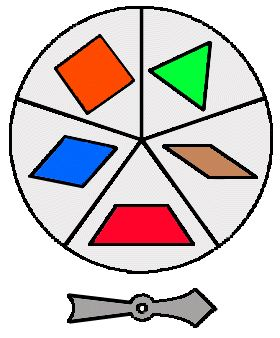
\includegraphics[width=1.25in,height=1.51in]{spinner.jpg}
\end{figure}
\FloatBarrier

\paragraph{Regression} This section will cover the concepts of scatterplots, best fit lines, Simpson's paradox, and regression to the mean. \\

\problem The goal of this is to learn how to build least squared lines from scratch, make predictions, calculate probabilities of responses, and to be able to leverage the power of JMP. Download \texttt{phila\_housing.JMP} and load it up. This data set contains information related to house sales in Philadelphia and it has many variables. We are particularly interested in building a model that predicts house selling price (in dollars) using crime rate.

\benum
\easysubproblem What data types are the variables ``selling price'' and ``crime rate''?
\easysubproblem Define ``response variable'' and ``explanatory variable'' and explain why they are sometimes called ``dependent variable'' and ``independent variable'' respectively.
\easysubproblem Is this an observational study or an experiment? Explain your answer.
\easysubproblem In the model we wish to create, what is the response variable ($Y$) and what is the explanatory variable ($X$)?
\easysubproblem Create a scatterplot using ``Fit Y by X'' for ``selling price'' and ``crime rate''. Analyze this scatterplot using the four criteria we went over in class (see bottom of p.108 for a refresher).
\easysubproblem Would you think it's appropriate to fit a line to this plot?
\easysubproblem Now, let JMP compute the univariate and bivariate statistics for you by clicking the red down arrow, then ``density ellipse'' and click the 0.95 option. Write down $\xbar, \ybar, s_x, s_y, r$.
\easysubproblem One of the rows was excluded from the data set (in JMP it appears with a cancel icon in the row header). Why is this row an outlier? To answer this question, un-exclude the row and create a new scatterplot, then explain what you see.
\easysubproblem Without using JMP, compute the best fit line's intercept ($b_0$) and slope ($b_1$) using the formulas from class and the univariate and bivariate statistics you wrote down previously.
\easysubproblem Use JMP to fit a least squares line by clicking the red down arrow and selecting the option ``Fit Line''. A line should appear as well as a bunch of information below the plot. Under the table header ``Linear Fit'', write down the equation. Is it the same as the one you came up with in the previous example? Print out this JMP analysis window and attach it to your homework.
\easysubproblem If the crime rate is 40, what is your best guess as to the sale price of the house?
\easysubproblem If the crime rate is 0, what is your best guess as to the sale price of the house?
\easysubproblem If the crime rate is 98.4, what is your best guess as to the sale price of the house?
\intermediatesubproblem Is there anything wrong with making the predictions in the previous two questions?
\easysubproblem Under the table header ``Summary of Fit'', write down the RMSE.
\intermediatesubproblem What is the probability of a house being worth more than \$200K if the crime rate is 30?
\intermediatesubproblem What is the probability of a house being worth less than \$200K if the crime rate is 35?
\hardsubproblem Consider the inverse problem where crime rate is viewed as a function of selling price. Use JMP to fit a least squares line for that data. Write down the equation. Now solve for selling price as a function of crime rate using that equation. Why is your equation different from the equation you got before?
\extracreditsubproblem Solve the following equation for $b_1$:

\beqn
\partialop{b_1}{\sumonen{i}{(y_i-\yhat_i)^2}} = 0
\eeqn

to prove that the slope estimate on the least squared line is: $b_1 = r\frac{s_y}{s_x}$. I showed you how to do this in class but I skipped over the messy details.
\eenum

\problem Now that you're a star in using JMP to create least squared regression lines, we will do another example. Download \texttt{doctor\_salary.JMP} and load it up. This dataset contains information about doctors and their salary. We are particulary interested in whether or not there is an effect of the number of publications on their salary.

\begin{figure}[htp]
\centering

\includegraphics[width=3in,height=1.82in]{doctor_salary.jpg}
\end{figure}
\FloatBarrier

\benum
\easysubproblem Create a best fit line for salary in 2005 explained by publications per year using the JMP methods you learned in the last problem. Write down the prediction equation.
\easysubproblem Would you say there's an association between publications per year and salary in 2005? Does publishing less \textit{cause} the doctor to make more money?
\easysubproblem Now we want to do the same analysis as before for each department the doctor is in. In JMP you would do this by doing a ``Fit Y by X'' where Y is salary in 2005, X is publications per year, and you would add Dept as the ``By'' variable. You should get 6 different scatterplots: one for each department. Fit a line to each of them. Do you see the negative association anymore? Is this an example of Simpson's paradox in action?
\intermediatesubproblem Why was there a negative association in part (a)? Explain it by using what you learned in part (c).
\eenum


\problem The method of creating a least squared line was named after the discovery of regression to the mean by Sir Francis Galton in the late 1800's. We will analyze a portion of Galton's original parent-child height dataset using \texttt{R}. Download the file \texttt{galton.RData} from webcafe and load it into \texttt{R} by using ``file...Load Workspace''. None of the code in the question will work without this since the file contains the dataset. The two variables are ``parent'' and ``child''. The parent variable is an average of the two parents' heights in inches (the mother's height was multiplied by 1.08 to adjust for gender differences). The child variable is the height of a child. The number of rows is $n=928$.

\begin{figure}[htp]
\centering
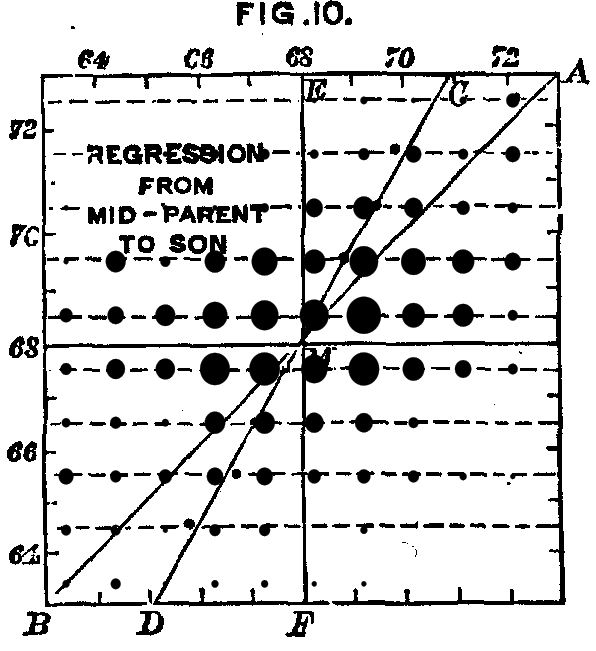
\includegraphics[width=2in,height=2.18in]{galton.jpg}
\caption{A table from Galton's original paper}
\end{figure}
\FloatBarrier

\benum
\easysubproblem Explain in your own words what ``regression toward the mean'' means.
\easysubproblem Run the following \texttt{R} code:

\begin{verbatim}
plot(galton$child, 
  galton$parent, 
  xlim = c(60, 75),
  ylim = c(60, 75),
  ylab = "Child Height (in)", 
  xlab = "Parent Height avg and adj (in)", 
  main = "Child Height vs Parent Height");
#end of code placeholder
\end{verbatim}

This will create a scatterplot. Use the criteria we discussed in class to describe the association in this plot.

\easysubproblem Explain what regression toward the mean would mean in this example. Do this before you do the next question.

\easysubproblem Run the following \texttt{R} code:

\begin{verbatim}
mod = lm(galton$child ~ galton$parent);
mod$coefficients;
#end of code placeholder
\end{verbatim}

From the output of above, write down the least squares regression line with the values substituted for $b_0$ and $b_1$, the intercept and slope.

\easysubproblem Now run the following \texttt{R} code:

\begin{verbatim}
abline(mod, col = "red");
abline(a = 0, b = 1, col = "blue");
#end of code placeholder
\end{verbatim}

This will draw in \inred{red} the least squares line on the plot and in \inblue{blue} the 45$^o$ line. This was one of the ways Galton originally studied regression to the mean. Do you see what he was surprised about? Explain.
\eenum

\paragraph{More Hypothesis Testing} This will be good practice for two-sample t-tests. This section is \textit{not required to hand in} but is strongly recommended. \\

\problem Amtrak maintains FRA Class 8 track on the NE corridor from Philadelphia to New York as well as other places. Class 8 track means it allows for top speeds of 125MPH on straightaways and 80MPH on turns. In order to run trains that quickly, the lines must maintain 10,000V AC which is converted to 6,500V DC to power the engines.

\begin{figure}[htp]
\centering
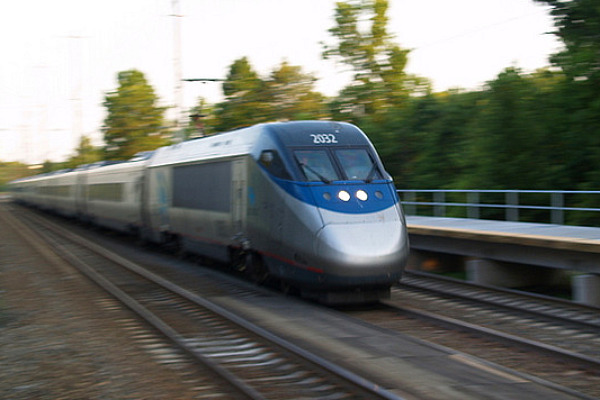
\includegraphics[width=2.5in,height=1.67in]{amtrak.jpg}
\end{figure}
\FloatBarrier

Sometimes voltages vary between stations. There are many reasons for such variation which are complicated. 12 samples were taken at New York Penn Station with a sample average of $9932$V and a sample standard deviation of $1232$V. 10 samples were taken at 30th Street Station in Philadelphia with an average of $9982$V with a standard deviation of $705$V.

\benum
\easysubproblem We are interested if there is a difference between the mean voltage at New York Penn station and at Philadelphia 30th Street Station. State hypotheses for the appropriate test.
\intermediatesubproblem Are there any problems with running this test?
\intermediatesubproblem Regardless of whether or not you thought there were problems, Run this test at $\alpha = 5\%$ disregarding the problems, if they exist.
\intermediatesubproblem In order to do a 2-sample $t$-test, you must first check to see if the standard deviations should be pooled or left unpooled. Make sure you did this in the previous part. You should have used the unpooled protocol. However, the ratio of the sample variances was very near 3. Run the test again at the same $\alpha$ level using the pooled. Did your answer change much?
\eenum

\end{document}
